Le projet de simulation Multi-Agents s'est porté sur le choix d'une adaptation d'\emph{Alien Versus Predator} car il permet d'introduire des règles complexes au sein d'un environnement assez simple. Tout l'intêret du projet est la définition des règles déterministes du jeu pour chacun des agents afin de le faire évouluer à partir d'un état initial.

\subsection{Conception des règles}

Nous avons voulu commencer par des règles simples que nous voulions complexifier par la suite grâce à des ajouts dans le code de contraintes pour chaque Agent. Les règles simples qui constituent la base du code sont les suivantes :
\begin{enumerate}
  \item Les Aliens tuent les Humains.
  \item Les Humains tuent les Prédators.
  \item Les Prédators tuent les Aliens.
\end{enumerate}

Ces règles permettent un certain équilibre dans le programme et chaque entité a ses chances de gagner la battaille pour la survie de sa race.

À cela j'ai ajouté un certain nombre de règle supplémentaire pour chaque agent :
\begin{itemize}
  \item Chaque agent vieillit à chaque tour et peut mourir de vieillesse à partir du 30\textsuperscript{ième} tour.
  \item Chaque agent a une majorité sexuelle fixé à 15 ans, \textit{c'est-à-dire} qu'il ne peut se reproduire qu'à partir de cet âge.
  \item Chaque agent a un champs de vision : chacun de leur déplacement sera fait en fonction de ce qu'il observe autour de lui. Le champ de vision amène ici un déséquilibre entre les entités puisque le Prédator a un champ de vision fixé à 6 cases tandis que les humains voient à 3 cases et les Aliens à 4 cases.
  \item Chaque entité a des points de vie afin qu'elle puisse survivre aux attaques et prévoir certaines interractions lorsqu'un agent est blessé. Cependant, pour les besoins du deboguage et par soucis de simplification du code chaque attaque tue directement la cible de cette attaque.
\end{itemize}

\subsection{Principe de la simulation}
Le terrain de jeu est une matrice déterminée selon les paramètres d'entrée du programme. C'est avec ces paramètres que cette matrice est crée, selon les types des Agents, cette création se fait via la methode :

\begin{lstlisting}[style=c++]
/**
 * Initialize the matrix of Agents.
 */
void DataStorage::initMatrix()
{
	double random;
	_matrix = new Agent**[_width];

	for (int i = 0 ; i < _width ; ++i)
	{
		_matrix[i] = new Agent*[_height];
		for (int j = 0 ; j < _height ; ++j)
		{
			random = GameController::getInstance()->getRandom();
			if (random < PROPORTIONS_CUMULEES[0])
            {
				_matrix[i][j] = new Alien(i,j);
            }
			else if (random < PROPORTIONS_CUMULEES[1])
            {
				_matrix[i][j] = new Human(i,j);
            }
			else if (random < PROPORTIONS_CUMULEES[2])
            {
				_matrix[i][j] = new Predator(i,j);
            }
			else
            {
				_matrix[i][j] = NULL;
            }
            
			if (_matrix[i][j])
            {
                _agents.push_back(_matrix[i][j]);
            }
		}
	}
}
\end{lstlisting}

La création du terrain de jeu se fait via le tirage d'un nombre aléatoire selon une table de répartition. Selon cette table de répartition et le tirage de nombre aléatoire entre 1 et 0 on peut déterminer si la case du terrain de jeu est un Agent (Alien, Prédator et Human) ou si c'est une case vide.
\begin{figure}[h]
\centering
\begin{multicols}{2}
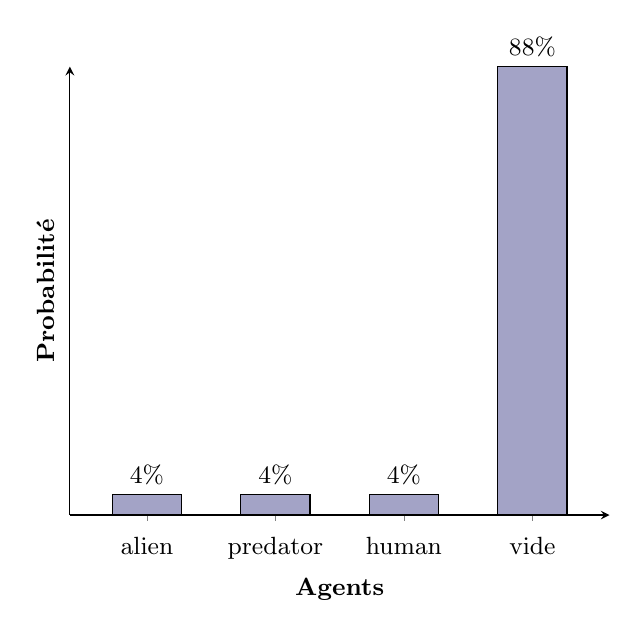
\begin{tikzpicture}[font=\small]
    \begin{axis}[
      ybar,
      bar width=25pt,
      xlabel={\bfseries Agents},
      ylabel={\bfseries Probabilité},
      ymin=0,
      ytick=\empty,
      xtick=data,
      axis x line=bottom,
      axis y line=left,
      enlarge x limits=0.2,
      symbolic x coords={alien,predator,human,vide},
      xticklabel style={anchor=base,yshift=-\baselineskip},
      nodes near coords={\pgfmathprintnumber\pgfplotspointmeta\%}
    ]
      \addplot[fill=MidnightBlue!40] coordinates {
        (alien,4)
        (predator,4)
        (human,4)
        (vide,88)
      };
    \end{axis}
  \end{tikzpicture}

\begin{tabular}{c}
  \textit{Table cumulant} \\
  \textit{les répartitions} \\
  \hline
  \hline
  1 \\
  0,12 \\
  0,08 \\
  0,04 \\ \hline
\end{tabular}

\end{multicols}
\caption{Distribution des agents dans la matrice de jeu.}
\end{figure}

\newpage
Le même principe est appliqué pour la création des comportements de chaque Agent. Un nombre aléatoire est tiré et selon une table des répartition que j'ai fixé arbitrairement afin d'équilibrer le déroulement de la simulation, chaque agent se voit attribuer un comportement qui déterminera ses actions au cours du tour de la simulation.

\begin{figure}[h]
\centering
\begin{multicols}{2}
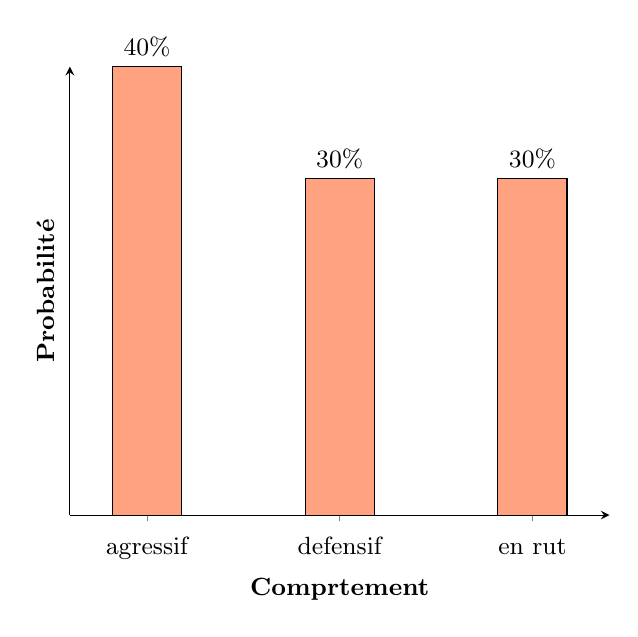
\begin{tikzpicture}[font=\small]
    \begin{axis}[
      ybar,
      bar width=25pt,
      xlabel={\bfseries Comprtement},
      ylabel={\bfseries Probabilité},
      ymin=0,
      ytick=\empty,
      xtick=data,
      axis x line=bottom,
      axis y line=left,
      enlarge x limits=0.2,
      symbolic x coords={agressif,defensif,en rut},
      xticklabel style={anchor=base,yshift=-\baselineskip},
      nodes near coords={\pgfmathprintnumber\pgfplotspointmeta\%}
    ]
      \addplot[fill=OrangeRed!50] coordinates {
        (agressif,40)
        (defensif,30)
        (en rut,30)
      };
    \end{axis}
  \end{tikzpicture}

\begin{tabular}{c}
  \textit{Table cumulant} \\
  \textit{les répartitions} \\
  \hline
  \hline
  1 \\
  0,7 \\
  0,3 \\ \hline
\end{tabular}

\end{multicols}
\caption{Distribution des actions pour chaque agent.}
\end{figure}